\newpage
\section{Use Case Skizzen}
\subsection{Akteure}
\begin{tabularx}{\linewidth}{X X}
\textbf{Akteur} & \textbf{Ziel}\\
\hline
\textbf{Public User} &
Registrieren
\\
\hline
\textbf{Registered User} & 
\textbf{Wenn User:}

Login

Logout

Service anlegen (Create)

Service Infos lesen (Read)

Service ändern (Update)

Service löschen (Delete)

Benutzerinfos ändern

\textbf{Wenn Admin:}

Benutzer anlegen

Benutzer löschen

Benutzer ändern

Benutzerinfos ändern

\\
\hline
\textbf{Cloud Anbieter} &
Service anlegen (Create)

Service Infos lesen (Read)

Service ändern (Update)

Service löschen (Delete)
\\

\end{tabularx}


\subsection{Use Case Diagramm}
\begin{figure}[!htbp]
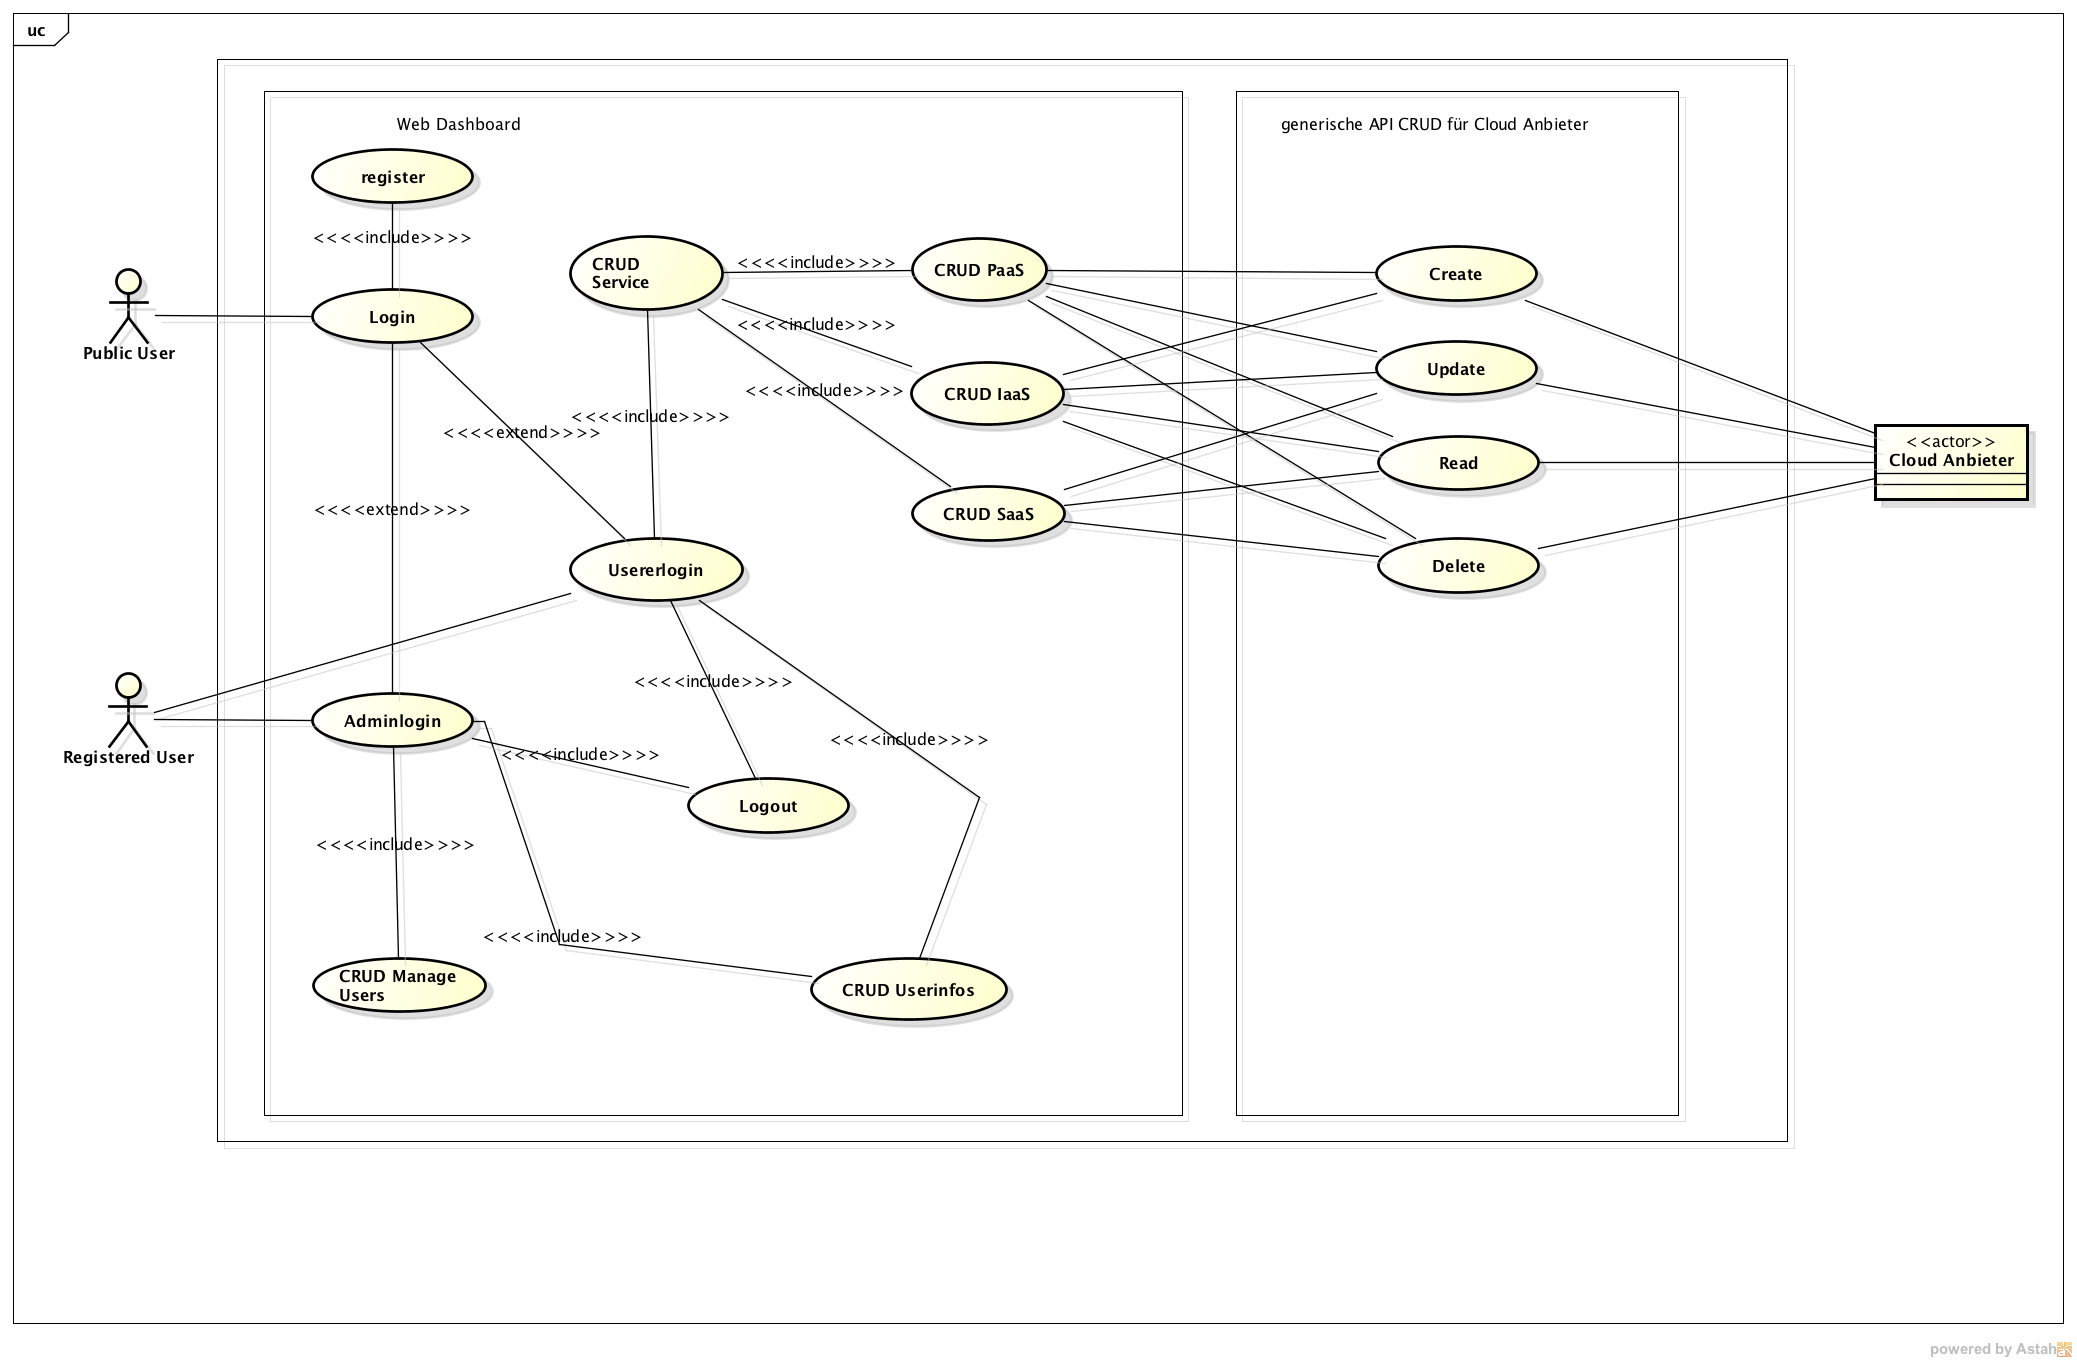
\includegraphics[width=\textwidth]{./03_Analyse/04_UseCases/images/UseCase-Skizzen}
\caption{Use Case Diagramm Skizze}
\end{figure}
